\chapter{Evaluation}

This chapter reports the evaluation results and interprets them in the scope
defined by Chapter 3.

\section{Evaluation Summary}

The main evaluation source is the report benchmark campaign, with a companion
operations campaign under the same harness policy defined in Chapter~3. All
listed targets succeeded, and this chapter applies Chapter~3's interpretation
rules when discussing smaller timing deltas.

\section{Objective to Evidence Traceability}

Table~\ref{tab:evaluation-traceability} maps the measurable objectives from
Table~\ref{tab:measurable-objectives} to the evidence used for final evaluation.
This is the central traceability table for the dissertation: each success claim
should connect to a run artifact, implementation target, or security chapter.

\begin{table}[H]
\centering
\scriptsize
\begin{tabular}{p{0.08\linewidth}p{0.21\linewidth}p{0.29\linewidth}p{0.18\linewidth}}
\hline
Objective & Evidence & Result & Status \\
\hline
O1 & Repository targets and harness JSON output & AES, Salsa20, LowMC,
operation suite, CTR, and CTR+HMAC targets emit benchmark records with success
status and metrics & Achieved for implemented target set \\
O2 & Main and operations benchmark campaigns & Headline tables and figures are
backed by aggregate summaries, per-trial records, logs, and generated plot data
& Partial (directional timing evidence) \\
O3 & LowMC/AES comparison and optimisation delta & Chapter~5 supports AES as the
final primitive; LowMC optimisation helped locally but did not close the
VM-level gap & Achieved as stack-specific result \\
O4 & Matched CTR and CTR+HMAC targets at 1, 4, 16, and 64 blocks & HMAC adds
user-cycle work at every tested block size; full-receipt size increases by 768
bytes & Achieved for implemented sizes \\
O5 & Chapters 10, 12, and 14 & Threat model, assumptions, game sketch,
limitations, and follow-up work are explicit & Partial (proof sketch, not full
formal proof) \\
\hline
\end{tabular}
\caption{Objective-to-evidence-to-result traceability table.}
\label{tab:evaluation-traceability}
\end{table}

\section{Authenticated Pipeline Performance}

Table~\ref{tab:ctr-and-ctrhmac-performance} reports the matched CTR-only and
CTR+HMAC performance rows used for the authenticated-pipeline comparison.

\begin{table}[H]
\centering
\scriptsize
\begin{tabular}{lrrrr}
\hline
Target & Prove s (median) & Verify s (median) & Total s (median) & User cycles (median) \\
\hline
\texttt{aes-ctr-1blk} & 7.4268 & 0.0104 & 7.4373 & 52945 \\
\texttt{aes-ctr-4blk} & 15.7277 & 0.0112 & 15.7390 & 159941 \\
\texttt{aes-ctr-16blk} & 64.4969 & 0.0127 & 64.5096 & 587806 \\
\texttt{aes-ctr-64blk} & 160.3976 & 0.0366 & 160.4341 & 2299177 \\
\hline
\texttt{aes-ctr-hmac-1blk} & 7.4239 & 0.0105 & 7.4344 & 79499 \\
\texttt{aes-ctr-hmac-4blk} & 14.9068 & 0.0111 & 14.9179 & 186756 \\
\texttt{aes-ctr-hmac-16blk} & 64.2531 & 0.0124 & 64.2655 & 615606 \\
\texttt{aes-ctr-hmac-64blk} & 157.4952 & 0.0361 & 157.5313 & 2330973 \\
\hline
\end{tabular}
\caption{Performance summary for CTR-only and CTR+HMAC targets.}
\label{tab:ctr-and-ctrhmac-performance}
\end{table}

Figure~\ref{fig:ctr-time-vs-blocks} plots the corresponding AES-CTR total-time
trend across the headline block sizes.

\begin{figure}[t]
\centering
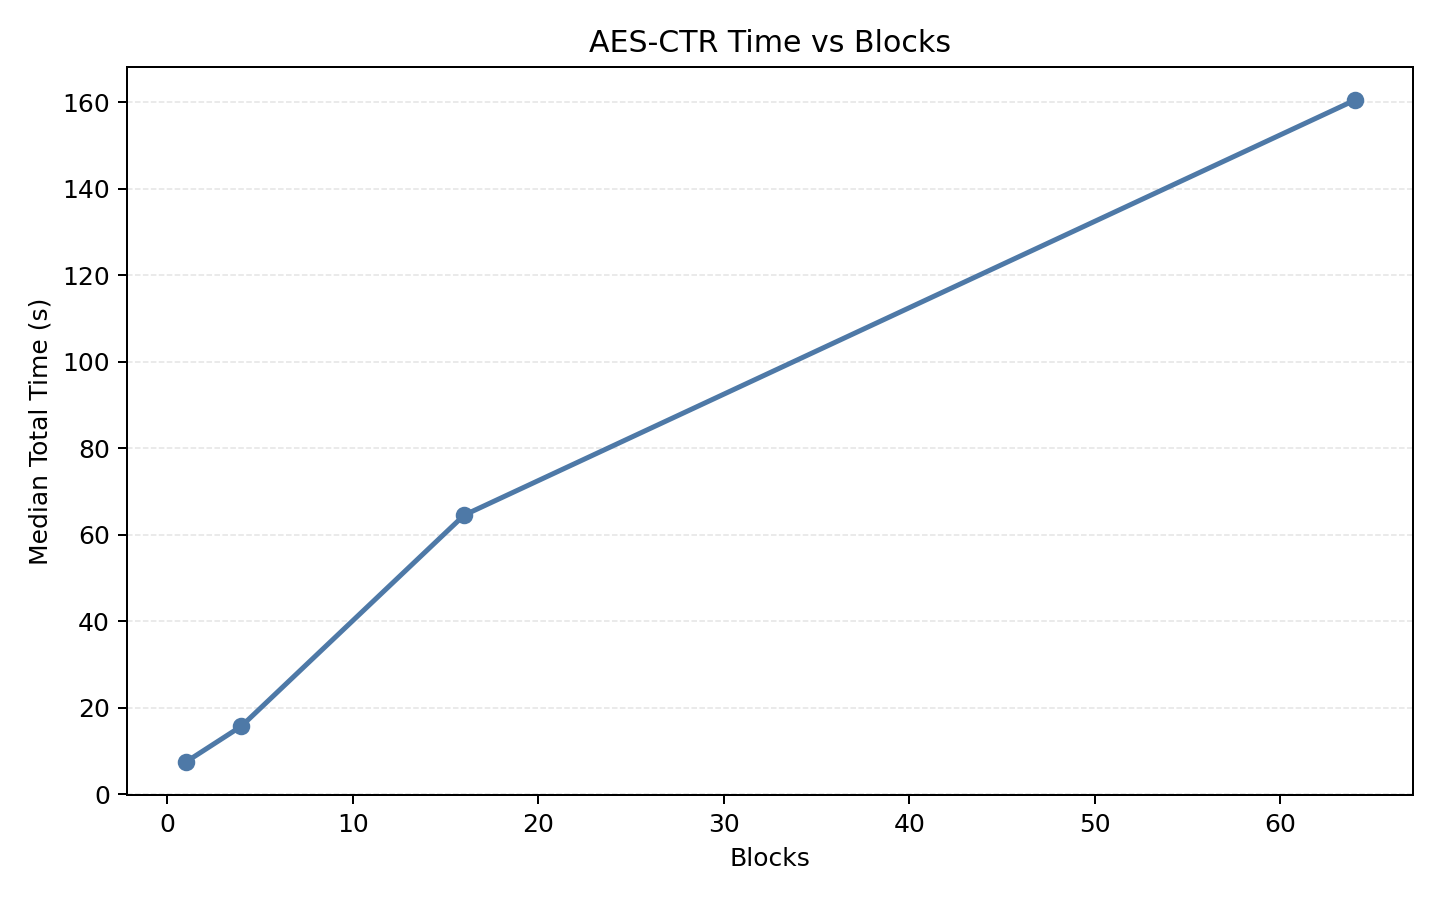
\includegraphics[width=0.82\linewidth]{Figures/report-benchmarks/ctr_time_vs_blocks.png}
\caption{AES-CTR median total time versus block count from the report benchmark run.}
\label{fig:ctr-time-vs-blocks}
\end{figure}

\section{Cycle Interpretation and Trace Rounding}

Three cycle views are used together when interpreting zkVM benchmark behavior:

\begin{itemize}
\item \textbf{Guest cycles (\(C_{user}\))}: a proxy for algorithm-efficiency in
guest code;
\item \textbf{Trace cycles (\(C_{total}\))}: the execution trace size that is
actually proven;
\item \textbf{Prover work (\(t_{prove}\))}: the wall-clock cost paid by the prover.
\end{itemize}

RISC Zero documents cycles and execution traces as the relevant cost surface for
guest programs, and its STARK protocol is built from polynomial encodings and
FRI-style low-degree testing \cite{risczeroTraceDocs,bensasson2018stark}.
In the benchmark data, this appears as power-of-two \(C_{total}\) buckets, so the
evaluation treats trace rounding as an observed proof-system load effect rather
than as native CPU timing behavior.

To make this visible in this repository, AES-CTR was run at every block count
from 1 through 16 in a block-count sweep. Figure~\ref{fig:ctr-trace-rounding-1-to-16} shows the
expected pattern: guest cycles increase roughly linearly with workload,
trace-cycle totals jump at power-of-two boundaries (\(2^{17}\), \(2^{18}\),
\(2^{19}\), \(2^{20}\)), and proving time steps up when the rounded trace size
crosses those boundaries.

\begin{figure}[t]
\centering
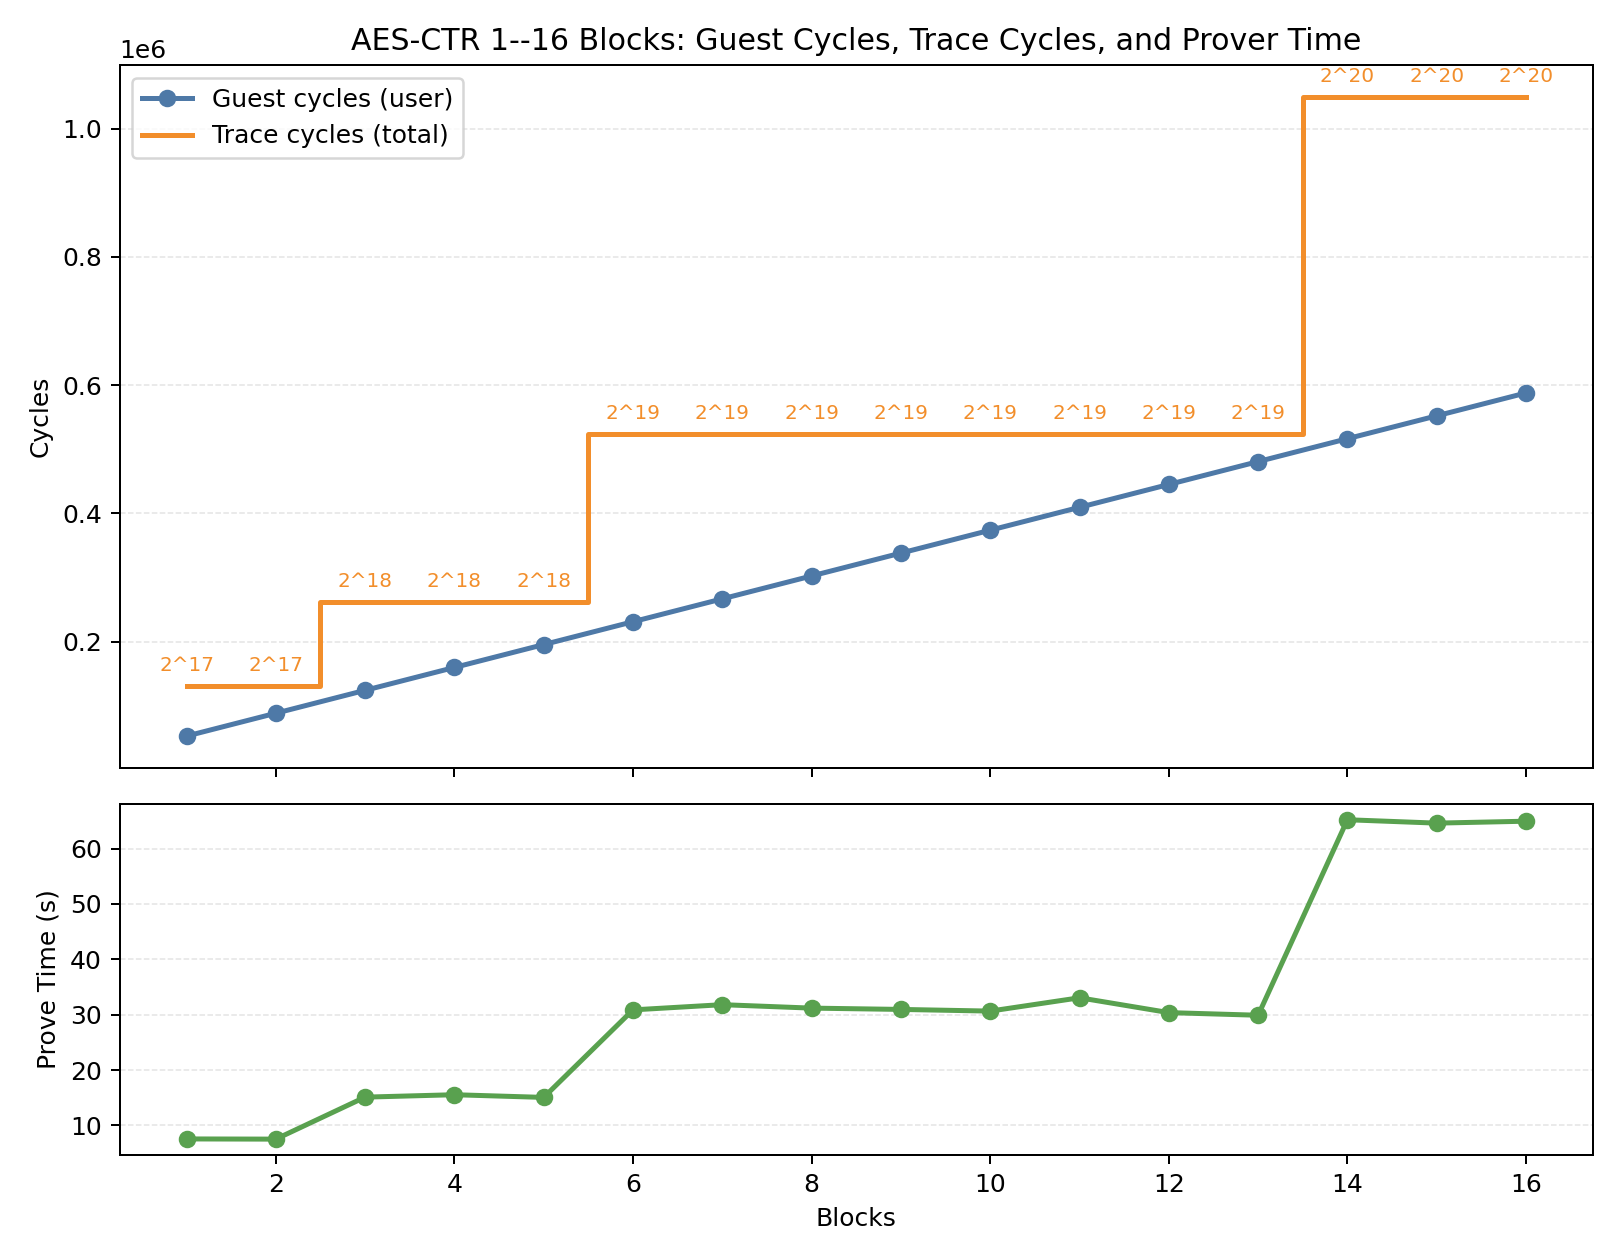
\includegraphics[width=0.88\linewidth]{Figures/report-benchmarks/ctr_trace_rounding_1_to_16.png}
\caption{AES-CTR block sweep (1--16 blocks): guest cycles rise with workload, while rounded trace cycles move in power-of-two steps that drive prover-time jumps.}
\label{fig:ctr-trace-rounding-1-to-16}
\end{figure}

In this sweep, rounded trace cycles stay at \(131072\) for 1--2 blocks,
\(262144\) for 3--5 blocks, \(524288\) for 6--13 blocks, and
\(1048576\) for 14--16 blocks. The prove-time curve follows the same
step pattern.

\section{Authentication Overhead (CTR vs CTR+HMAC)}

Table~\ref{tab:auth-overhead-deltas} reports the matched deltas used to separate
wall-clock noise from the more stable user-cycle overhead signal.

\begin{table}[H]
\centering
\small
\begin{tabular}{rrrrr}
\hline
Blocks & Total s delta & Total s delta \% & User-cycle delta & User-cycle delta \% \\
\hline
1 & -0.0029 & -0.04\% & +26554 & +50.15\% \\
4 & -0.8211 & -5.22\% & +26815 & +16.77\% \\
16 & -0.2441 & -0.38\% & +27800 & +4.73\% \\
64 & -2.9029 & -1.81\% & +31796 & +1.38\% \\
\hline
\end{tabular}
\caption{CTR+HMAC overhead relative to CTR from benchmark results. Negative
total-time deltas reflect wall-clock noise rather than a real speed-up from
authentication; user-cycle deltas are the more reliable overhead signal and are
positive for every block size (see discussion below).}
\label{tab:auth-overhead-deltas}
\end{table}

The cycle signal is consistent: CTR+HMAC adds user-cycle work at every block
size. Total-time deltas are noisier and occasionally negative, so cycle deltas
are treated as the more robust overhead indicator.

The significance of this result is that authentication overhead is visible in
the execution trace even when wall-clock timing is unstable. User cycles increase
by about 26--32 thousand cycles across the tested payloads, while the percentage
overhead falls as block count grows because fixed authentication work is
amortized over a larger encryption workload. This is the expected direction for
a fixed framing and tag computation cost.

The negative wall-clock deltas do not mean HMAC makes proving faster. They show
that wall-clock values are too noisy for small mode-family deltas. For design
conclusions, the report therefore uses total time mainly for large effects and
user cycles for explaining smaller structural overheads.

Figure~\ref{fig:auth-overhead-ctr-vs-hmac} visualizes the same CTR+HMAC overhead
pattern across matched block sizes.

\begin{figure}[t]
\centering

\includegraphics[width=0.86\linewidth]{Figures/report-benchmarks/auth_overhead_ctr_vs_ctr_hmac.png}
\caption{CTR+HMAC overhead relative to CTR across matched block sizes.}
\label{fig:auth-overhead-ctr-vs-hmac}
\end{figure}

\section{Proof-Size Reporting}

Table~\ref{tab:proof-size-summary} reports the proof-size fields used to separate
proof payload changes from computation overhead.

\begin{table}[H]
\centering
\small
\begin{tabular}{lrrr}
\hline
Blocks & CTR proof bytes & CTR+HMAC proof bytes & Full-receipt delta (HMAC-CTR) \\
\hline
1 & 243944 & 243944 & +768 \\
4 & 255656 & 255656 & +768 \\
16 & 281128 & 281128 & +768 \\
64 & 830136 & 830136 & +768 \\
\hline
\end{tabular}
\caption{Proof-size summary from benchmark results.}
\label{tab:proof-size-summary}
\end{table}

In this dataset, seal size is unchanged by adding HMAC, while full receipt size
increases by a small constant amount.

This matters because it separates computation overhead from proof payload
overhead. Adding HMAC changes guest work, as shown by user cycles, but does not
change the seal-size field in the benchmark dataset. In these measurements, the
constant full-receipt increase is consistent with additional journal/output
material rather than a large proof-system size penalty for the HMAC computation
itself.

\section{LowMC Evaluation Inserts}

LowMC-specific values are interpreted using the detailed comparison in
Chapter~5. As reported in Figure~\ref{fig:lowmc-vs-aes-prove} and
Table~\ref{tab:lowmc-baseline-vs-optimised}, optimisation improved LowMC
materially but did not close the VM-level gap to AES.

This remains the strongest empirical result in the dissertation because the
effect-size gap is much larger than the small mode-family timing deltas in the
authenticated-overhead table. It therefore supports the final AES selection more
strongly than any wall-clock difference in the authenticated-pipeline comparison.

\section{Evaluation Relative to Related Work}

Circuit-oriented literature motivates LowMC and other ZK-friendly primitives by
nonlinear/constraint efficiency \cite{albrecht2015ciphers,jaques2019grover}.
This project's evaluation adds a different perspective: under a concrete zkVM
software stack, trace-composition and implementation overhead can dominate and
reverse expected rankings \cite{risczeroTraceDocs}.

In that sense, the dissertation does not challenge the prior circuit-level
results; it qualifies their transferability to VM-based proving workflows.

Compared with related work, the contribution is not a new cipher design or a
better circuit construction. It is an empirical systems result: a primitive
chosen for low nonlinear complexity can still perform poorly when implemented as
ordinary guest software in a zkVM. The evaluation therefore connects literature
expectations to deployment evidence, rather than treating circuit and VM cost
models as interchangeable.

\section{Statistical Validity}

The validity rule used in this chapter follows Chapter~3: large ratios can
support broad ranking, while small timing differences need cycle-level support.
The main interpretation pattern is effect-size sensitivity:

\begin{itemize}
\item large ratios, such as LowMC versus AES proving time, are treated as robust
directional findings;
\item small total-time differences, especially negative HMAC deltas, are treated
as noise-prone and not used as standalone conclusions;
\item cycle differences are used to explain execution-structure changes because
they are less dependent on scheduler and thermal variation than wall-clock time.
\end{itemize}

Chapter~13 gives the stronger rerun and artifact-provenance roadmap.

\section{Failure and Edge-Case Analysis}

No listed target in the main and operations campaigns failed, timed out, or
produced parse errors. This supports the reliability of the reported values, but
it does not exhaustively test all adversarial inputs.

The most important edge cases are:

\begin{itemize}
\item very small payloads, where fixed prover and receipt overhead dominate;
\item larger payloads, where block-count scaling becomes the main cost driver;
\item authenticated-mode mismatches, where AAD, IV, ciphertext, tag, or key
changes should fail before plaintext is trusted;
\item receipt or image-ID mismatch, where the host should reject the transcript
independently of cryptographic byte formatting.
\end{itemize}

The current report evaluates the first two through block-size sweeps and treats
the latter two through design and security analysis. A fuller test campaign would
add explicit negative-path integration tests for each authenticated mismatch.

\section{Reflection: Achievements and Gaps}

What went well:

\begin{itemize}
\item a reproducible harness and artifact pipeline were established and used
consistently across chapters;
\item the final authenticated pipeline was implemented end-to-end within the
local benchmark/proof workflow, with proof verification and explicit mode-family
separation;
\item the central empirical finding (AES outperforming LowMC in this zkVM stack)
is supported by receipt-backed measurements.
\end{itemize}

What did not fully meet the ideal target:

\begin{itemize}
\item statistical confidence remains limited for small timing deltas;
\item commit-hash embedding in run artifacts is incomplete;
\item cross-zkVM replication is not yet available.
\end{itemize}

Follow-up work should strengthen the benchmark campaign and artifact provenance
before making broader claims. Chapter~13 details that roadmap.
